\section{Einführung}
\label{sec:Einfuehrung}
In Zeiten der Digitalisierung des Öffentlichen Verkehrs wird umso mehr Software benötigt die gewisse Bedürfnisse befriedigt. Seit 2016 stellt die Plattform\footnote{\url{https://opentransportdata.swiss/}} aktuelle Datensätze für den Öffentlichen Verkehr der Schweiz zur Verfügung. Die Daten umfassen Fahrplandaten, Echtzeitdaten, Statistische Daten und noch mehr. Daraus lassen sich Programme realisieren wie z.B. ein Journey Planner der Verbindungsvorschläge inkl.Umsteigvorgänge erstellt. 

\subsection{Aufgabenstellung}
\label{Aufgabenstellung}
Für das Projekt "Massgeschneiderte online buchbare Angebote für Gruppenreisen" wird eine Distanzmetrik zwischen geografischen Punkten benötigt um Unterkünfte zu finden, welche "nahe" bei touristischen Attraktionen liegen. Die einfachste Methode wäre die Luftliniendistanz zu berechnen. Hat aber den Nachteil das geographische Unebenheiten wie Tal und Bergspitze als eben angesehen werden, oder z.b. geographische Probleme mit Seen die umfahren werden müssen etc. So würden Distanz von Unterkünften zu Attraktionen fälschlicherweise als nah erkannt werden. Nun stehen Daten vom Öffentlichen Verkehr zur Verfügung um dieses Problem zu lösen.

\subsection{Vorgehen}
\label{Vorgehen}
In dieser Arbeit werden wir also die Datensätze analysieren, die von der Plattform zur Verfügung stehen,um herauszufinden welche Datensätze wir benötigen. Aber vor allem muss ein Algorithmus gefunden und eventuell angepasst werden der diese Aufgabe zur vollster Zufriedenheit löst. Um daraus einen Journey-Planner zu entwickeln.



\subsection{Ziel der Bachelorarbeit}
\label{Ziel der Bachelorarbeit}
\begin{figure}[]
	\centering
	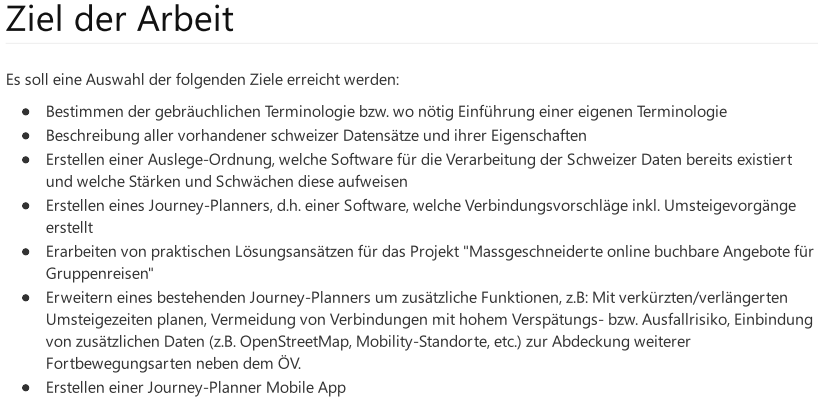
\includegraphics[width=15cm]{Zielderarbeit.png}
	\caption{Dies sind die möglichen Ziele für die Bachelorarbeit. Aus dieser offenen Aufgabenstellung werden wir im verlaufe dieses Berichts eine eigene ausgearbeitete Aufgabenstellung erarbeiten.}
	\label{fig:Ziel der Arbeit}
\end{figure}

\begin{figure}[]
	\centering
	
\includegraphics[width=15cm]{Aufgabenstellungfachmodul.png}
	\caption{Dies sind unsere Ziele die wir in der Arbeit am Fachmodul zu berücksichtigen haben. }
	\label{fig:Aufgabenstellung Fachmodul}
\end{figure} Bachelorarbeit}